\documentclass[number]{ximera}

%My github password is ximera1
%My GeoGebra password is Ximera1

%\usepackage{tikz}

\renewcommand{\theenumi}{\arabic{enumi}.}


% set font encoding for PDFLaTeX, XeLaTeX, or LuaTeX
\usepackage{ifxetex,ifluatex}
\newif\ifxetexorluatex
\ifxetex
  \xetexorluatextrue
\else
  \ifluatex
    \xetexorluatextrue
  \else
    \xetexorluatexfalse
  \fi
\fi

\ifxetexorluatex
  \usepackage{fontspec}
\else
  \usepackage[T1]{fontenc}
  \usepackage[utf8]{inputenc}
  \usepackage{lmodern}
\fi

\usepackage{hyperref}
\usepackage{tikz} %% Adding this here so it's not manually added elsewhere

% set font encoding for PDFLaTeX, XeLaTeX, or LuaTeX
%\usepackage{ifxetex,ifluatex}
%\newif\ifxetexorluatex
%\ifxetex
%  \xetexorluatextrue
%\else
%  \ifluatex
%    \xetexorluatextrue
%  \else
%    \xetexorluatexfalse
%  \fi
%\fi
%
%\ifxetexorluatex
%  \usepackage{fontspec}
%\else
%  \usepackage[T1]{fontenc}
%  \usepackage[utf8]{inputenc}
%  \usepackage{lmodern}
%\fi
%
%\usepackage{hyperref}

\usepackage{tikz}

\renewcommand{\theenumi}{\arabic{enumi}.}

\title{Area of a Triangle}
\author{Univ. of Minnesota MathCEP}


% Enable SageTeX to run SageMath code right inside this LaTeX file.
% http://mirrors.ctan.org/macros/latex/contrib/sagetex/sagetexpackage.pdf
% \usepackage{sagetex}

\begin{document}

\begin{abstract}
  In this activity, you will discover additional formulas for calculating the area of a triangle in the SAS case and in the cases when two angles and a side length are given. 
The SSS case can be done in a similar manner, though the most common form, called {\it{Heron's Formula}} is not easily derived.
\end{abstract}

\maketitle

Assume we know the formula for the area of a triangle

$$Area \; = \; \frac{1}{2}(base)(height)$$


The following problems are about SAS triangles, in which we are given the lengths of two sides and the angle between them.
Pay attention to the process you use to solve for $h$ and the area of the triangle.

Note that $b$ is the entire length from $A$ to $C$, not just the portion that would be the adjacent side to angle $A$ in the right triangle.

\begin{problem}
Given $b = 7$, $c=5$ and $A = 35^\circ$, find $h$ and the area of the triangle.
\begin{image}
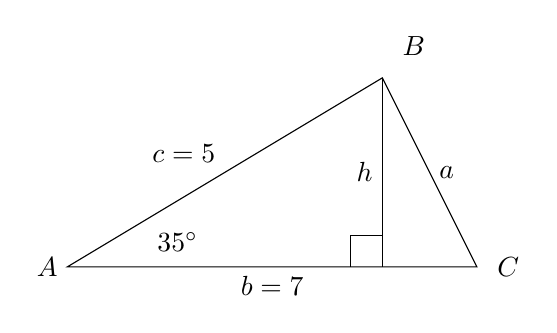
\begin{tikzpicture}[scale=4]
\draw node[left]{$A$} (0,0) -- node[below] {$b=7$} (1.3,0) -- node[right] {$a$}  (1,0.6) -- node[above left] {$c=5$} (0,0) -- cycle;
\draw (1,0.6) -- node[left]{$h$} (1,0);
\draw (0.9,0.1) -- (0.9,0);
\draw (0.9,0.1) -- (1,0.1);
\node at (1.1,0.7) {$B$};
\node at (1.4,0) {$C$};
\node at (0.35,0.08) {$35^\circ$};
\end{tikzpicture}
\end{image}
$h=\answer[tolerance=0.1]{5\sin(35\pi/180)}$

Area = $\answer[tolerance=0.1]{35\sin(35\pi/180)/2}$ %Can we accept rounded answers?

\begin{hint}
If $\sin(35^\circ)=\frac{h}{5}$, what is $h$?
\end{hint}
\end{problem}

\begin{problem}
Given $b = 12$, $c=8$ and $A = 52^\circ$, find $h$ and the area of the triangle.

$h=\answer[tolerance=0.1]{8\sin(52\pi/180)}$

Area $=\answer[tolerance=0.1]{12*8\sin(52\pi/180)/2}$
\end{problem}

\begin{problem}
Given $b = 4$, $c=11$ and $A = 83^\circ$, find $h$ and the area of the triangle.

$h=\answer[tolerance=0.1]{11\sin(83\pi/180)}$

Area $=\answer[tolerance=0.1]{4*11\sin(83\pi/180)/2}$
\end{problem}

\begin{problem}
Given $b = 10$, $c=9$ and $A = 115^\circ$, find $h$ and the area of the triangle.

$h=\answer[tolerance=0.1]{9\sin(115\pi/180)}$

Area $=\answer[tolerance=0.1]{10*9\sin(115\pi/180)/2}$
\end{problem}

\begin{question}
Describe, in words, the steps needed to find the area of a triangle, given $A$, $b$, and $c$. (You may also use mathematical expressions in your description.)
\begin{freeResponse}
\end{freeResponse}
\end{question}


\begin{question}
Using $c$ and $A$, write a formula for $h$. Then write a formula for the area of the triangle. 
\begin{image}
 \begin{tikzpicture}[scale=4]


\draw node[left]{$A$} (0,0) -- node[below] {$b$} (1.3,0) -- node[right] {$a$}  (1,0.6) -- node[above left] {$c$} (0,0) -- cycle;

\draw (1,0.6) -- node[left]{$h$} (1,0);
\draw (0.9,0.1) -- (0.9,0);
\draw (0.9,0.1) -- (1,0.1);
\node at (1.1,0.7) {$B$};
\node at (1.4,0) {$C$};
 \end{tikzpicture}
\end{image}

$h=\answer{c\sin(A)}$

Area $=\answer{\frac{bc\sin(A)}{2}}$

\begin{hint}
Your answers should be in terms of angle $A$ and side lengths $b$ and $c$.
\end{hint}
\end{question}

\begin{question}
Repeat using $a$ and $C$. That is, using $a$ and $C$, write a formula for $h$. Then write a formula for the area of the triangle.

$h=\answer{a\sin(C)}$

Area $=\answer{\frac{ab\sin(C)}{2}}$

\begin{hint}
Your answers should be in terms of angle $C$ and side lengths $a$ and $b$.
\end{hint}
\end{question}


In the following problems, you are provided with two angles and a side length.
Because the angles of a triangle must add up to $180^\circ$, knowing two angles implies that you know the third angle.
For this reason, the formula you are about to derive will work for AAS and ASA triangles.
In each case find $c$, then find $h$, then find the area of the triangle.

 Note that $b$ is the entire length from $A$ to $C$, not just the portion that would be the adjacent side to angle $A$ in the right triangle.


\begin{problem}
Given $b = 7$, $A = 35^\circ$, $B = 65^\circ$ and $C = 80^\circ$
\begin{image}
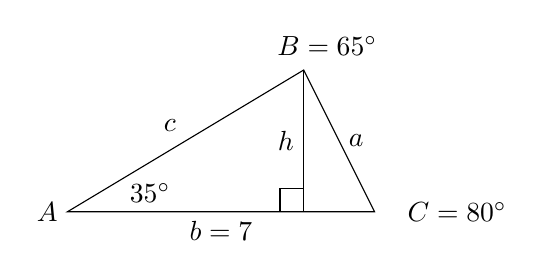
\begin{tikzpicture}[scale=3]

\draw node[left]{$A$} (0,0) -- node[below] {$b=7$} (1.3,0) -- node[right] {$a$}  (1,0.6) -- node[above left] {$c$} (0,0) -- cycle;

\draw (1,0.6) -- node[left]{$h$} (1,0);
\draw (0.9,0.1) -- (0.9,0);
\draw (0.9,0.1) -- (1,0.1);
\node at (1.1,0.7) {$B=65^\circ$};
\node at (1.65,0) {$C=80^\circ$};
\node at (0.35,0.08) {$35^\circ$};

\end{tikzpicture}
\end{image}

$c=\answer[tolerance=0.1]{7\sin(80\pi/180)/\sin(65\pi/180)}$

\begin{hint}
Apply the Law of Sines using $b$, $B$, and $C$.
\end{hint}

$h=\answer[tolerance=0.1]{7\sin(80\pi/180)\sin(35\pi/180)/(\sin(65\pi/180))}$

\begin{hint}
In the first part of this activity, you were able to solve for $h$ given angle $A$ and side length $c$.
How can you apply that idea to the side length $c$ you solved for above?
\end{hint}

Area $= \answer[tolerance=0.1]{7^2\sin(80\pi/180)\sin(35\pi/180)/(2\sin(65\pi/180))}$
\end{problem} 

\begin{problem} 
Given $b = 12$, $A = 52^\circ$, $B = 67^\circ$ and $C = 61^\circ$

$c=\answer[tolerance=0.1]{12\sin(61\pi/180)/\sin(67\pi/180)}$

$h=\answer[tolerance=0.1]{12\sin(61\pi/180)\sin(52\pi/180)/\sin(67\pi/180)}$

Area $=\answer[tolerance=0.1]{12^2\sin(61\pi/180)\sin(52\pi/180)/(2\sin(67\pi/180))}$
\end{problem}

\begin{problem}
Given $b = 5$, $A = 85^\circ$, $B = 23^\circ$ and $C = 72^\circ$

$c=\answer[tolerance=0.1]{5\sin(72\pi/180)/\sin(23\pi/180)}$

$h=\answer[tolerance=0.1]{5\sin(72\pi/180)\sin(85\pi/180)/\sin(23\pi/180)}$

Area $=\answer[tolerance=0.1]{5^2\sin(72\pi/180)\sin(85\pi/180)/(2\sin(23\pi/180))}$
\end{problem}

\begin{problem}
Given $b = 11$, $A = 115^\circ$, $B = 43^\circ$ and $C = 22^\circ$

$c=\answer[tolerance=0.1]{11\sin(22\pi/180)/\sin(43\pi/180)}$

$h=\answer[tolerance=0.1]{11\sin(22\pi/180)\sin(115\pi/180)/\sin(43\pi/180)}$

Area $=\answer[tolerance=0.1]{11^2\sin(22\pi/180)\sin(115\pi/180)/(2\sin(43\pi/180))}$
\end{problem}

\begin{question} 
Describe, in words, the steps needed to find the area of a triangle, given $b$, $A$, $B$, and $C$. (You may also use mathematical expressions in your description.)
\begin{freeResponse}
\end{freeResponse}
\end{question}


\begin{question}
 Derive a formula for the area of a triangle, given $b$, $A$, $B$ and $C$, by doing the following:

\begin{image}
 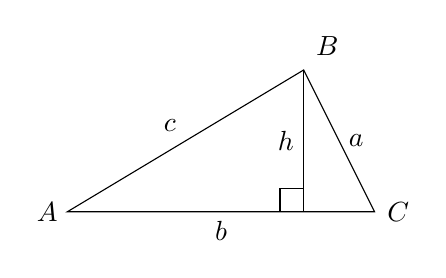
\begin{tikzpicture}[scale=3]


\draw node[left]{$A$} (0,0) -- node[below] {$b$} (1.3,0) -- node[right] {$a$}  (1,0.6) -- node[above left] {$c$} (0,0) -- cycle;

\draw (1,0.6) -- node[left]{$h$} (1,0);
\draw (0.9,0.1) -- (0.9,0);
\draw (0.9,0.1) -- (1,0.1);
\node at (1.1,0.7) {$B$};
\node at (1.4,0) {$C$};
 \end{tikzpicture}

\end{image}
 
\begin{enumerate}
\item Find $c$, as a function of $b$, $C$ and $B$:

$c=\answer{\frac{b\sin(C)}{\sin(B)}}$

\item Find $h$, as a function of $c$ and $A$:

$h=\answer{c\sin(A)}$

\item Find $h$, as a function of $b$, $A$, $B$ and $C$:

$h=\answer{\frac{b\sin(C)\sin(A)}{\sin(B)}}$

\begin{hint}
Replace $c$ in the equation above with your expression for $c$ from the start of this Question.
\end{hint}

\item Find the area of the triangle, as a function of $b$, $A$, $B$ and $C$:

Area $= \answer{\frac{b^2\sin(C)\sin(A)}{2\sin(B)}}$

\end{enumerate}

\end{question}

\begin{question}
Can you use the equation above to find the area of an $AAA$ triangle?
\begin{multipleChoice}
\choice{Always}
\choice{Sometimes, depending on what the angles are}
\choice[correct]{Never}
\end{multipleChoice}
\end{question}

 \end{document}

